%% For double-blind review submission, w/o CCS and ACM Reference (max submission space)
\documentclass[sigplan,9pt,review,anonymous]{acmart}\settopmatter{printfolios=true,printccs=false,printacmref=false}
%% For double-blind review submission, w/ CCS and ACM Reference
%\documentclass[sigplan,10pt,review,anonymous]{acmart}\settopmatter{printfolios=true}
%% For single-blind review submission, w/o CCS and ACM Reference (max submission space)
%\documentclass[sigplan,10pt,review]{acmart}\settopmatter{printfolios=true,printccs=false,printacmref=false}
%% For single-blind review submission, w/ CCS and ACM Reference
%\documentclass[sigplan,10pt,review]{acmart}\settopmatter{printfolios=true}
%% For final camera-ready submission, w/ required CCS and ACM Reference
%\documentclass[sigplan,10pt]{acmart}\settopmatter{}


%% Conference information
%% Supplied to authors by publisher for camera-ready submission;
%% use defaults for review submission.
\acmConference[LICS'18]{Logic in Computer Science}{July 09--12, 2018}{Oxford, UK}
\acmYear{2018}
\acmISBN{} % \acmISBN{978-x-xxxx-xxxx-x/YY/MM}
\acmDOI{} % \acmDOI{10.1145/nnnnnnn.nnnnnnn}
\startPage{1}

%% Copyright information
%% Supplied to authors (based on authors' rights management selection;
%% see authors.acm.org) by publisher for camera-ready submission;
%% use 'none' for review submission.
\setcopyright{none}
%\setcopyright{acmcopyright}
%\setcopyright{acmlicensed}
%\setcopyright{rightsretained}
%\copyrightyear{2017}           %% If different from \acmYear

%% Bibliography style
\bibliographystyle{ACM-Reference-Format}
%% Citation style
%\citestyle{acmauthoryear}  %% For author/year citations
%\citestyle{acmnumeric}     %% For numeric citations
%\setcitestyle{nosort}      %% With 'acmnumeric', to disable automatic
                            %% sorting of references within a single citation;
                            %% e.g., \cite{Smith99,Carpenter05,Baker12}
                            %% rendered as [14,5,2] rather than [2,5,14].
%\setcitesyle{nocompress}   %% With 'acmnumeric', to disable automatic
                            %% compression of sequential references within a
                            %% single citation;
                            %% e.g., \cite{Baker12,Baker14,Baker16}
                            %% rendered as [2,3,4] rather than [2-4].


%%%%%%%%%%%%%%%%%%%%%%%%%%%%%%%%%%%%%%%%%%%%%%%%%%%%%%%%%%%%%%%%%%%%%%
%% Note: Authors migrating a paper from traditional SIGPLAN
%% proceedings format to PACMPL format must update the
%% '\documentclass' and topmatter commands above; see
%% 'acmart-pacmpl-template.tex'.
%%%%%%%%%%%%%%%%%%%%%%%%%%%%%%%%%%%%%%%%%%%%%%%%%%%%%%%%%%%%%%%%%%%%%%


%% Some recommended packages.
\usepackage{tikz}
\usetikzlibrary{positioning}
\usepackage{stmaryrd}
\usepackage{multicol}
\usepackage{booktabs}   %% For formal tables:
                        %% http://ctan.org/pkg/booktabs
\usepackage{subcaption} %% For complex figures with subfigures/subcaptions
                        %% http://ctan.org/pkg/subcaption
\newcommand{\maps}{\colon}
\newcommand{\into}{\hookrightarrow}
\newcommand{\interp}[1]{\llbracket #1 \rrbracket}

\begin{document}

%% Title information
\title{Logic as a distributive law}         %% [Short Title] is optional;
                                        %% when present, will be used in
                                        %% header instead of Full Title.
%\titlenote{with title note}             %% \titlenote is optional;
                                        %% can be repeated if necessary;
                                        %% contents suppressed with 'anonymous'
%\subtitle{Subtitle}                     %% \subtitle is optional
%\subtitlenote{with subtitle note}       %% \subtitlenote is optional;
                                        %% can be repeated if necessary;
                                        %% contents suppressed with 'anonymous'


%% Author information
%% Contents and number of authors suppressed with 'anonymous'.
%% Each author should be introduced by \author, followed by
%% \authornote (optional), \orcid (optional), \affiliation, and
%% \email.
%% An author may have multiple affiliations and/or emails; repeat the
%% appropriate command.
%% Many elements are not rendered, but should be provided for metadata
%% extraction tools.

%% Author with single affiliation.
\author{Gregory Meredith}
%\authornote{with author1 note}          %% \authornote is optional;
                                        %% can be repeated if necessary
%\orcid{nnnn-nnnn-nnnn-nnnn}             %% \orcid is optional
\affiliation{
  \position{President}
%  \department{Department1}              %% \department is recommended
  \institution{RChain Cooperative}            %% \institution is required
%  \streetaddress{Street1 Address1}
  \city{Seattle}
  \state{WA}
%  \postcode{Post-Code1}
  \country{USA}                    %% \country is recommended
}
\email{lgreg.meredith@gmail.com}          %% \email is recommended

%% Author with two affiliations and emails.
\author{Michael Stay}
%%\authornote{with author2 note}          %% \authornote is optional;
                                        %% can be repeated if necessary
%%\orcid{nnnn-nnnn-nnnn-nnnn}             %% \orcid is optional
\affiliation{
  \position{Cofounder and CTO}
%%  \department{Department2a}             %% \department is recommended
  \institution{Pyrofex Corporation}           %% \institution is required
%%  \streetaddress{Street2a Address2a}
  \city{Orem}
  \state{UT}
%%  \postcode{Post-Code2a}
  \country{USA}                   %% \country is recommended
}
\email{stay@pyrofex.net}         %% \email is recommended


%% Abstract
%% Note: \begin{abstract}...\end{abstract} environment must come
%% before \maketitle command
\begin{abstract}
  Categorical logic focuses on structure-preserving functors from a ``syntactic'' category of formulae and proofs to a ``semantic'' category of realizations.  We show that in many interesting cases, this functor is a distributive law between monads.  The first monad $T$ describes the terms of a programming language, while the second monad $C$ describes a notion of collection.  Formulae are terms in $T+C$ while realizations are terms in $CT.$  Realization is a natural transformation defined in terms of the units and joins of the monads as well as a distributive law $\delta\maps TC \Rightarrow CT.$
  
  Finitary monads correspond to Lawvere theories. Mild generalizations of Lawvere theories capture not only term structure but also reduction relations. When we use these generalized Lawvere theories in the construction above, the resulting type system is both spatial and behavioral. It captures information both about the structure of the data being manipulated as well as about the possible evolutions of a term. Our main result is that the ``arrow'' type constructor in functional programming languages arises as a modality in the spatial-behavioral type system.
\end{abstract}


%% 2012 ACM Computing Classification System (CSS) concepts
%% Generate at 'http://dl.acm.org/ccs/ccs.cfm'.
\begin{CCSXML}
<ccs2012>
<concept>
<concept_id>10011007.10011006.10011008</concept_id>
<concept_desc>Software and its engineering~General programming languages</concept_desc>
<concept_significance>500</concept_significance>
</concept>
<concept>
<concept_id>10003456.10003457.10003521.10003525</concept_id>
<concept_desc>Social and professional topics~History of programming languages</concept_desc>
<concept_significance>300</concept_significance>
</concept>
</ccs2012>
\end{CCSXML}

\ccsdesc[500]{Software and its engineering~General programming languages}
\ccsdesc[300]{Social and professional topics~History of programming languages}
%% End of generated code


%% Keywords
%% comma separated list
\keywords{keyword1, keyword2, keyword3}  %% \keywords are mandatory in final camera-ready submission


%% \maketitle
%% Note: \maketitle command must come after title commands, author
%% commands, abstract environment, Computing Classification System
%% environment and commands, and keywords command.
\maketitle


\section{Introduction}
Every category has an associated internal logic.  The objects $X$ are thought of as collections of items of type $X;$ the morphisms $X \to Y$ are thought of as terms of type $Y$ with a single free variable of type $X.$  Subobjects $P \into X$ are thought of as predicates $P(X)$ that pick out those items in $X$ for which $P$ is true.

Computer programmers often use algebraic data types (ADTs) to describe collections, but ADTs do not explicitly specify a notion of morphism that we can use to define a subobject.  We could use a limits theory to explicitly describe a small category of structures and morphisms, but ADTs are defined recursively, and there's a clear notion of substructure as the structure at a recursion point.  For example, a subtree is a subterm of the term representing the tree.  In this paper, we only consider data types that are self-recursive rather than sets of types that are mutually recursive.

If we define a morphism from a term $X$ to a term $Y$ to be a choice of a copy of $X$ in $Y$, then all morphisms are monos.  With this choice of morphism, subobjects in the categorical sense correspond to subterms.

We can weaken the notion of subobject by considering a morphism from a term $X$ to a term $Y$ to be a choice of a copy of $X$ in $Y$ up to relabeling.  Relabeling equivalence classes are in one-to-one correspondence with terms labeled by the one-element set.  The type of unlabeled structures then often plays a role similar to the subobject classifier in a topos.  A subobject of $X$ in a topos corresponds to a morphism $X \to \Omega,$ where $\Omega$ is the subobject classifier.  Given the monad $C$ corresponding to our ADT encoding a notion of collection, we often have a transformation
\[ \phi_{X,Y}\maps C(X \times Y) \to (X \to CY) \]
natural in $Y$ and dinatural in $X$ that takes a collection of pairs and returns a function that maps each element of $X$ to the collection of $Y$ it was paired with.  $\phi_{X,1}$ maps $C(X) \cong C(X\times 1)$ to $X \to C1.$  When $C$ is the covariant powerset monad, the two concepts coincide.

\section{Formulae and realizability}

Types in computer programming describe collections of terms of the programming language.  Often, this is done by allowing type identifiers to appear in place of literals in the grammar.  For instance, in Facebook's Flow type system for JavaScript, we can replace the specific name and age in the record 
\begin{center}
  {\tt \{name: "Joe Schmoe", age: 45\}}
\end{center}
with the types {\tt string} and {\tt number}, respectively, to get a type of records:
\begin{center}
  {\tt \{name: string, age: number\}}.
\end{center}

This suggests that given an ADT $T$ describing terms in a programming language and an ADT $C$ describing a notion of collection, we can sum the two to get an ADT for formulae.  

The interpretation of a formula is a collection of terms.  A collection of terms is simply the composition of the two monads applied to the generators.  Therefore, we expect the interpretation of a formula to be given by a natural transformation
\[ \interp{-}\maps T+C \Rightarrow CT. \]
The natural transformation can be expressed in terms of the units and joins of $T$ together with a distributive law
\[ \delta\maps TC \Rightarrow CT. \]
We think of a collection as a way of ``summing'' terms together and the term constructors themsleves as a kind of formal product.  The distributive law maps products of sums to sums of products.

Such a distributive law may not always exist.  In figures 1 and 2, we show how the ``sets of'' collection monad admits both linear and nonlinear combinators, but the ``lists of'' collection monad only admits linear ones.

Given a distributive law $\delta\maps TC \Rightarrow CT$ and an algebra $(X, h\maps CTX \to X),$ we can compose them to get an algebra $(X, h\delta\maps (T+C)X \to X).$

\begin{figure*}
  \def\w{5}\def\h{2}
  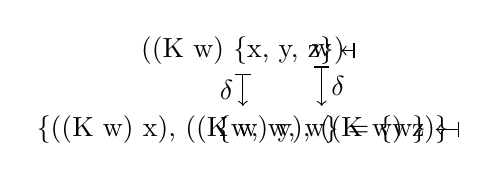
\begin{tikzpicture}
    \node (A) at (0,\h) {((K w) \{x, y, z\})};
    \node (B) at (\w,\h) {w}
      edge [<-|] (A);
    \node (C) at (0,0) {\{((K w) x), ((K w) y), ((K w) z)\}}
      edge [<-|] node [left] {$\delta$} (A);
    \node (D) at (\w,0) {\{w, w, w\} = \{w\}}
      edge [<-|] node [right] {$\delta$} (B)
      edge [<-|] (C);
  \end{tikzpicture}
  \def\w{8}\def\h{2}
  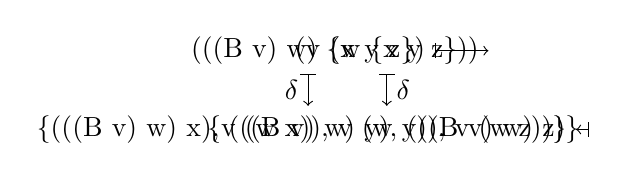
\begin{tikzpicture}
    \node (A) at (0,\h) {(((B v) w) \{x y z\})};
    \node (B) at (\w,\h) {(v (w \{x y z\}))}
      edge [<-|] (A);
    \node (C) at (0,0) {\{(((B v) w) x), (((B v) w) y), (((B v) w) z)\}}
      edge [<-|] node [left] {$\delta$} (A);
    \node (D) at (\w,0) {\{v (w x)), v (w y)), v (w z))\}}
      edge [<-|] node [right] {$\delta$} (B)
      edge [<-|] (C);
  \end{tikzpicture}
\caption{Using the ``sets of'' collection monad with the combinators $K$ and $B$.}
\end{figure*}




\begin{figure*}
\def\w{5}\def\h{2}
  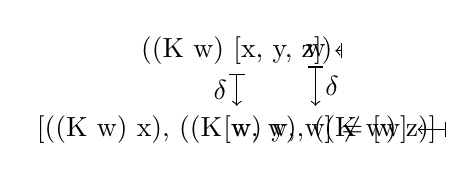
\begin{tikzpicture}
    \node (A) at (0,\h) {((K w) [x, y, z])};
    \node (B) at (\w,\h) {w}
      edge [<-|] (A);
    \node (C) at (0,0) {[((K w) x), ((K w) y), ((K w) z)]}
      edge [<-|] node [left] {$\delta$} (A);
    \node (D) at (\w,0) {[w, w, w] $\ne$ [w]}
      edge [<-|] node [right] {$\delta$} (B)
      edge [<-|] (C);
  \end{tikzpicture}

  \def\w{8}\def\h{2}
  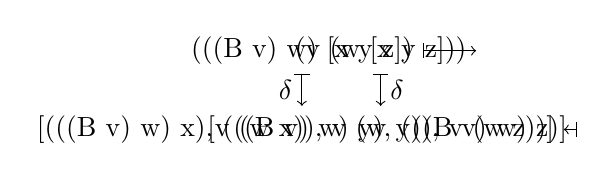
\begin{tikzpicture}
    \node (A) at (0,\h) {(((B v) w) [x y z])};
    \node (B) at (\w,\h) {(v (w [x y z]))}
      edge [<-|] (A);
    \node (C) at (0,0) {[(((B v) w) x), (((B v) w) y), (((B v) w) z)]}
      edge [<-|] node [left] {$\delta$} (A);
    \node (D) at (\w,0) {[v (w x)), v (w y)), v (w z))]}
      edge [<-|] node [right] {$\delta$} (B)
      edge [<-|] (C);
  \end{tikzpicture}
\caption{Using the ``lists of'' collection monad with the combinators $K$ and $B$.  Because $K$ discards information, there is no nontrivial distributive law for the $SKI$ calculus and the list monad.  The $BCI$ calculus, on the other hand, is linear, and works fine with the list monad.}
\end{figure*}

Given $\delta\maps T+C \Rightarrow CT$ and an algebra $h\maps CTX \to X,$ get algebra $h\delta_X\maps (T+C)X \to X.$


%% ∃_f S = [ y∈Y | ∃x∈X. f(x)=y  ∧  x∈S ] = map f S%% 
%% 
%% f:ℕ->[ℕ]%% 
%% f(x) = [x] if x even, [] otherwise%% 
%% How to write this?%% 
%% x is ``even'' if there exists y st y+y = x%% 
%% 
%% !:X -> 1%% 
%% exists_! S = [•∈1 | ∃x∈X. !(x) = •  ∧  x in S] = S nonempty%% 
%% 
%% S = [x'∈{x} | ∃y∈ℕ. y+y = x' ^ y∈ℕ ]%% 
%% 
%% evens in S⊆ℕ: join [ y∈Y | ∃x:ℕ. f(x) = y  ∧  x ∈ S ] = [y | x <- S, y <- f(x)] = flatmap f S%% 
%% 
%% inhabitation s in S = 1 if not, otherwise yes%% 
%% 
%% ``set-like'' collections: P1 is a classifier %% 
%% 


%% Acknowledgments
\begin{acks}                            %% acks environment is optional
                                        %% contents suppressed with 'anonymous'
\end{acks}


%% Bibliography
%\bibliography{bibfile}


%% Appendix
\appendix
\section{Appendix}

Text of appendix \ldots

\end{document}
